\section{Benutzertests}

Wie im Dokument ``Ergonomic Criteria for the Evaluation of Human-Computer Interfaces'' spezifiziert, stellt eine kriterienbasierte Bewertungsmethode lediglich einen analytischen Ansatz dar.
Als solche sind die Kriterien nicht dazu gedacht, andere Bewertungsmethoden zu ersetzen.
Daher sind Benutzertests weiterhin notwendig, um die Leistung und Nutzbarkeit einer Schnittstelle zu gewährleisten.
Aus diesem Grund wurden Benutzertests entwickelt, um allgemeine Usability-Probleme zu identifizieren und potenziell Probleme zu erkennen, die nicht von den Kriterien abgedeckt werden.

Das Ziel dieses Tests ist es, die Effektivität, Effizienz und Zufriedenheit mit der Silvanet-Webanwendung mithilfe von echten Nutzern zu quantifizieren.
Zunächst muss jedoch definiert werden, was getestet werden soll und vor allem, wie getestet werden soll.

\subsection{Festlegung der Testabdeckung}

Um relevante und schnelle Tests für die Benutzer durchführen zu können, mussten wir festlegen, auf welche Bereiche der Benutzeroberfläche sich die Tests konzentrieren sollten.
Es erschien uns sinnvoll, eine Gruppenaktivität mit dem Cloud-Team durchzuführen, um Ideen zu sammeln und die am meisten erwähnten auszuwählen.
Um die Brainstorming-Sitzung zu strukturieren und zu vermeiden, dass man sich zu sehr verzettelt, basiert die Aktivität auf der Ideationstechnik namens \textit{Lotus Blossoms}, die es ermöglicht, eine Idee nach der anderen gründlich zu erforschen.
Diese von S. Tatsuno 1990\cite{lotusBlossoms} entwickelte Methode der Ideenfindung lässt sich leicht durch das folgende Flussdiagramm schematisieren.

\begin{figure}[H]
  \centering
  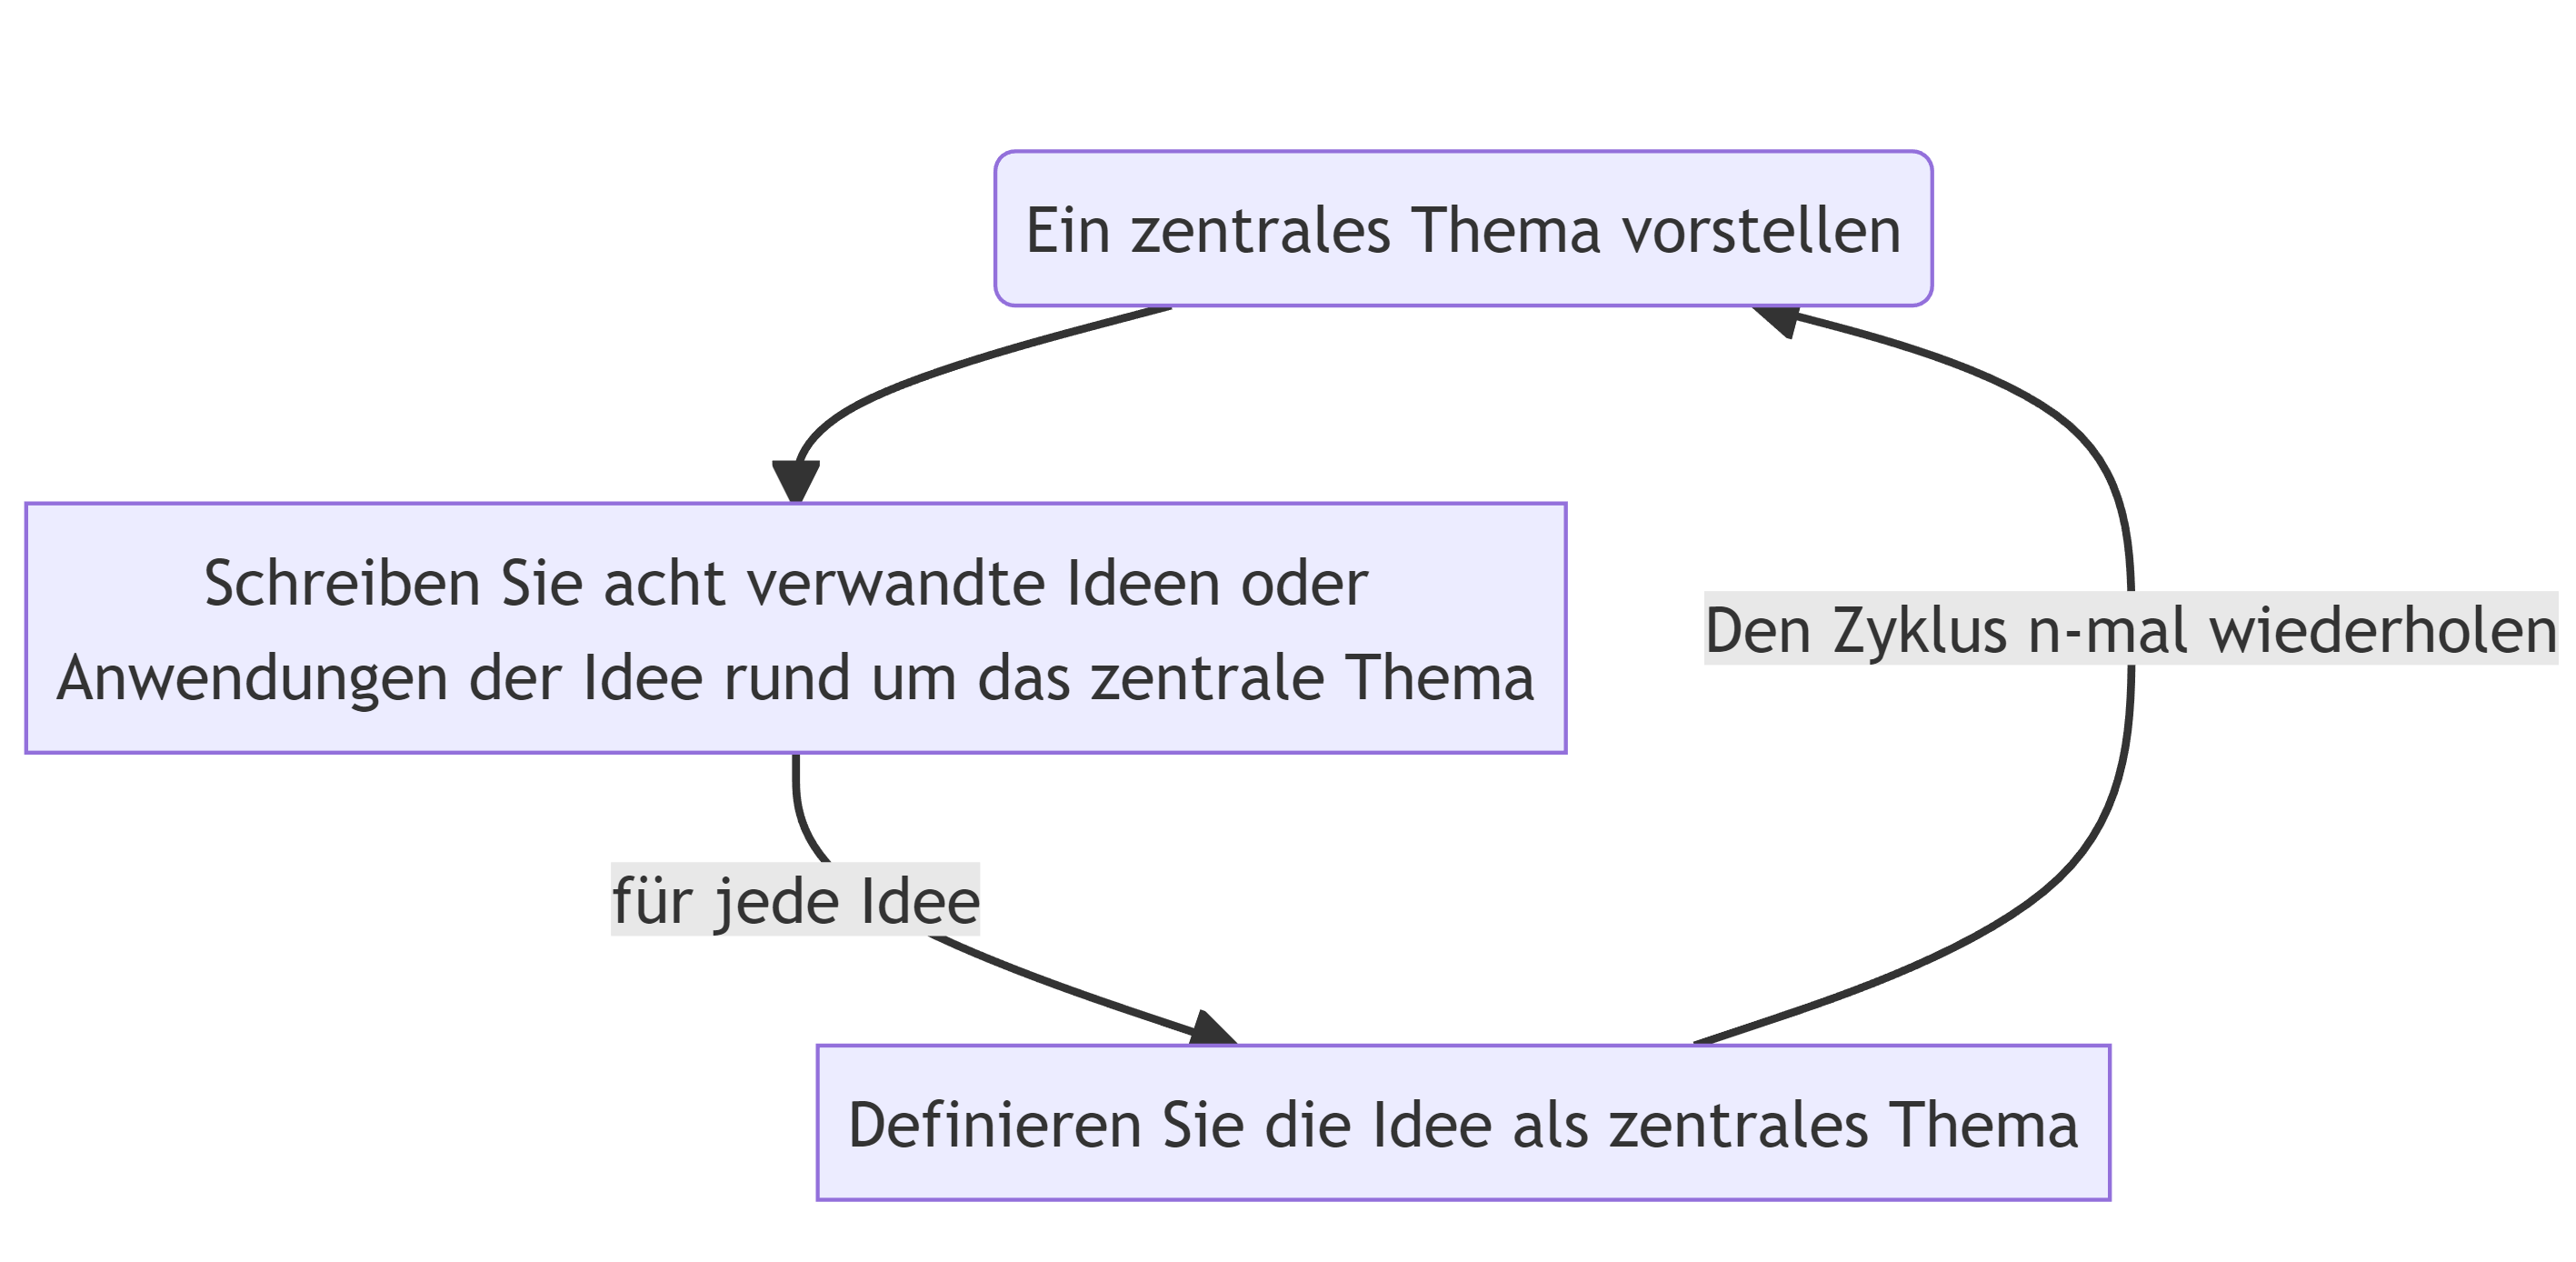
\includegraphics[width=\textwidth]{lotus_blossoms_flowdiagram}
  \caption{Darstellung eines Ideationszyklus mit der Lotus-Blossom-Methode}
  \label{fig:lotus_blossoms_flowdiagram}
\end{figure}

In diesem Fall sollte eine Iteration von zwei Zyklen ausreichen, um die wesentlichen Funktionen der Anwendung zu definieren.
Die erste zentrale Frage wurde im Vorfeld mit der Frage ``Was sind die Ziele des Gesprächs mit dem Kunden über die Anwendung?'' festgelegt.
Aus dieser Frage ergaben sich 6 verschiedene andere Themen:

\begin{itemize}
  \item Welche Informationen über die Geräte sind von Interesse?
  \item Ist die Planung eines \textit{Site} funktionsfähig und die Schnittstelle funktionstüchtig?
  \item Welche kundenorientierten Funktionen sollten den Nutzern zur Verfügung gestellt werden?
  \item Welche Art von Informationen würden Sie im Falle eines Feueralarms interessieren?
  \item Welche Art von Informationen möchten Sie auf dem Dashboard sehen?
  \item Funktioniert die Kartendarstellung gut?
\end{itemize}

\begin{figure}[H]
  \centering
  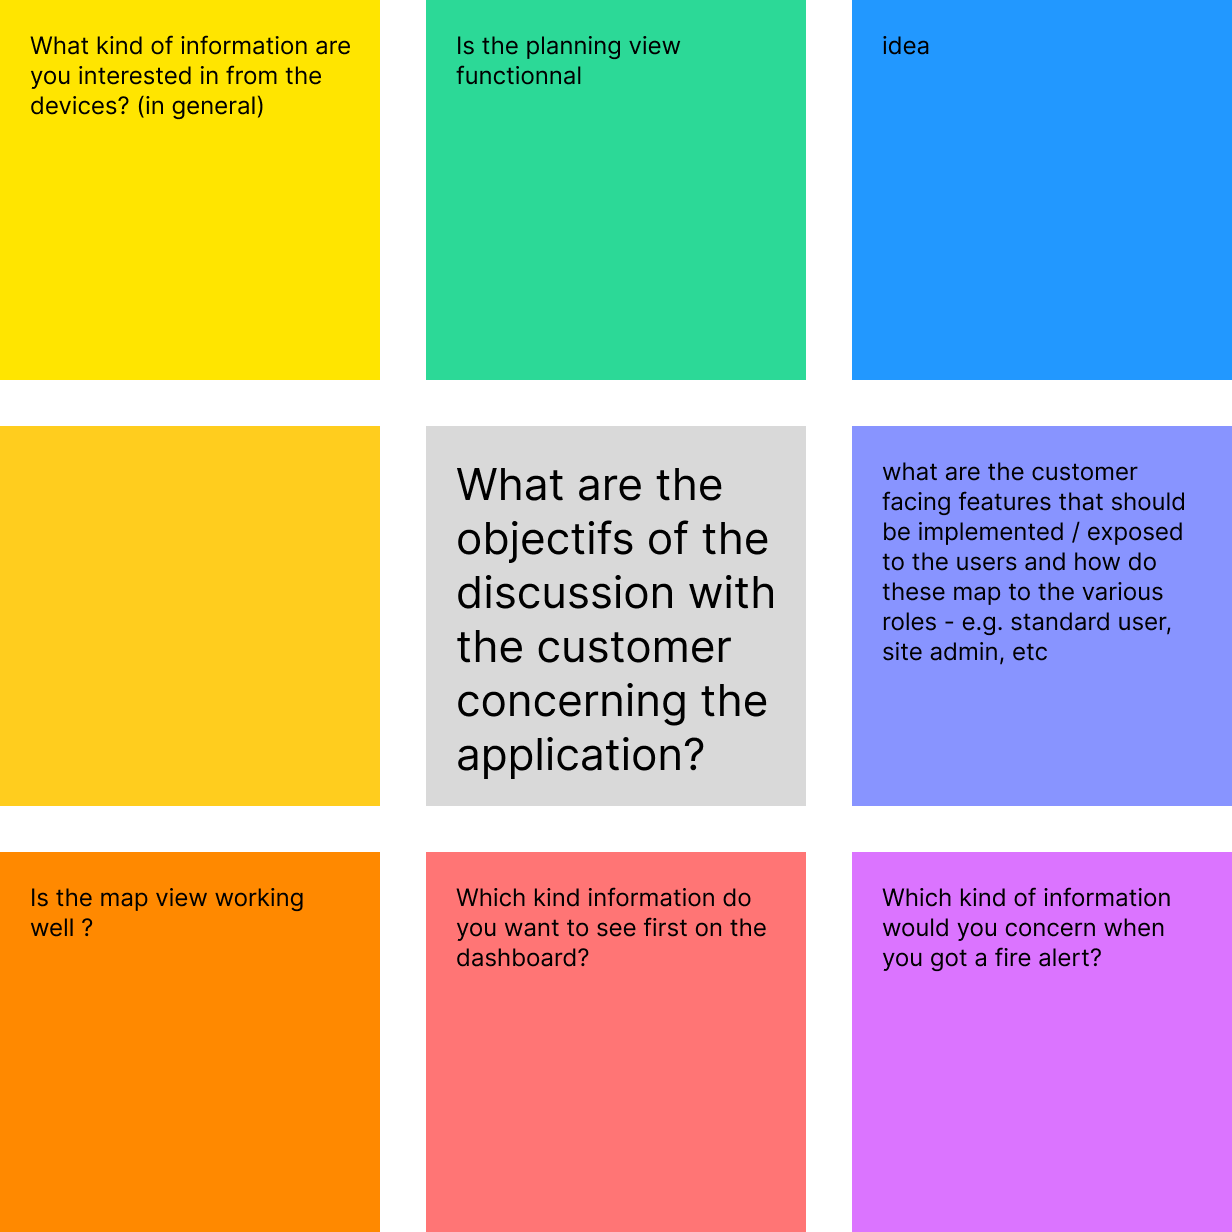
\includegraphics[width=10cm]{dryad_lotus_blossom_cycle_1}
  \caption{Durchführung des ersten Ideationszyklus durch das Cloud-Team von Dryad mit der Lotus-Blossom-Methode}
  \label{fig:dryad_lotus_blossom_cycle_1}
\end{figure}

In der zweiten Iteration wurden mehr Fragen zu den Funktionen der Benutzeroberfläche gestellt, die die genannten Themen beantworten oder näher erläutern können.

\begin{figure}[H]
  \centering
  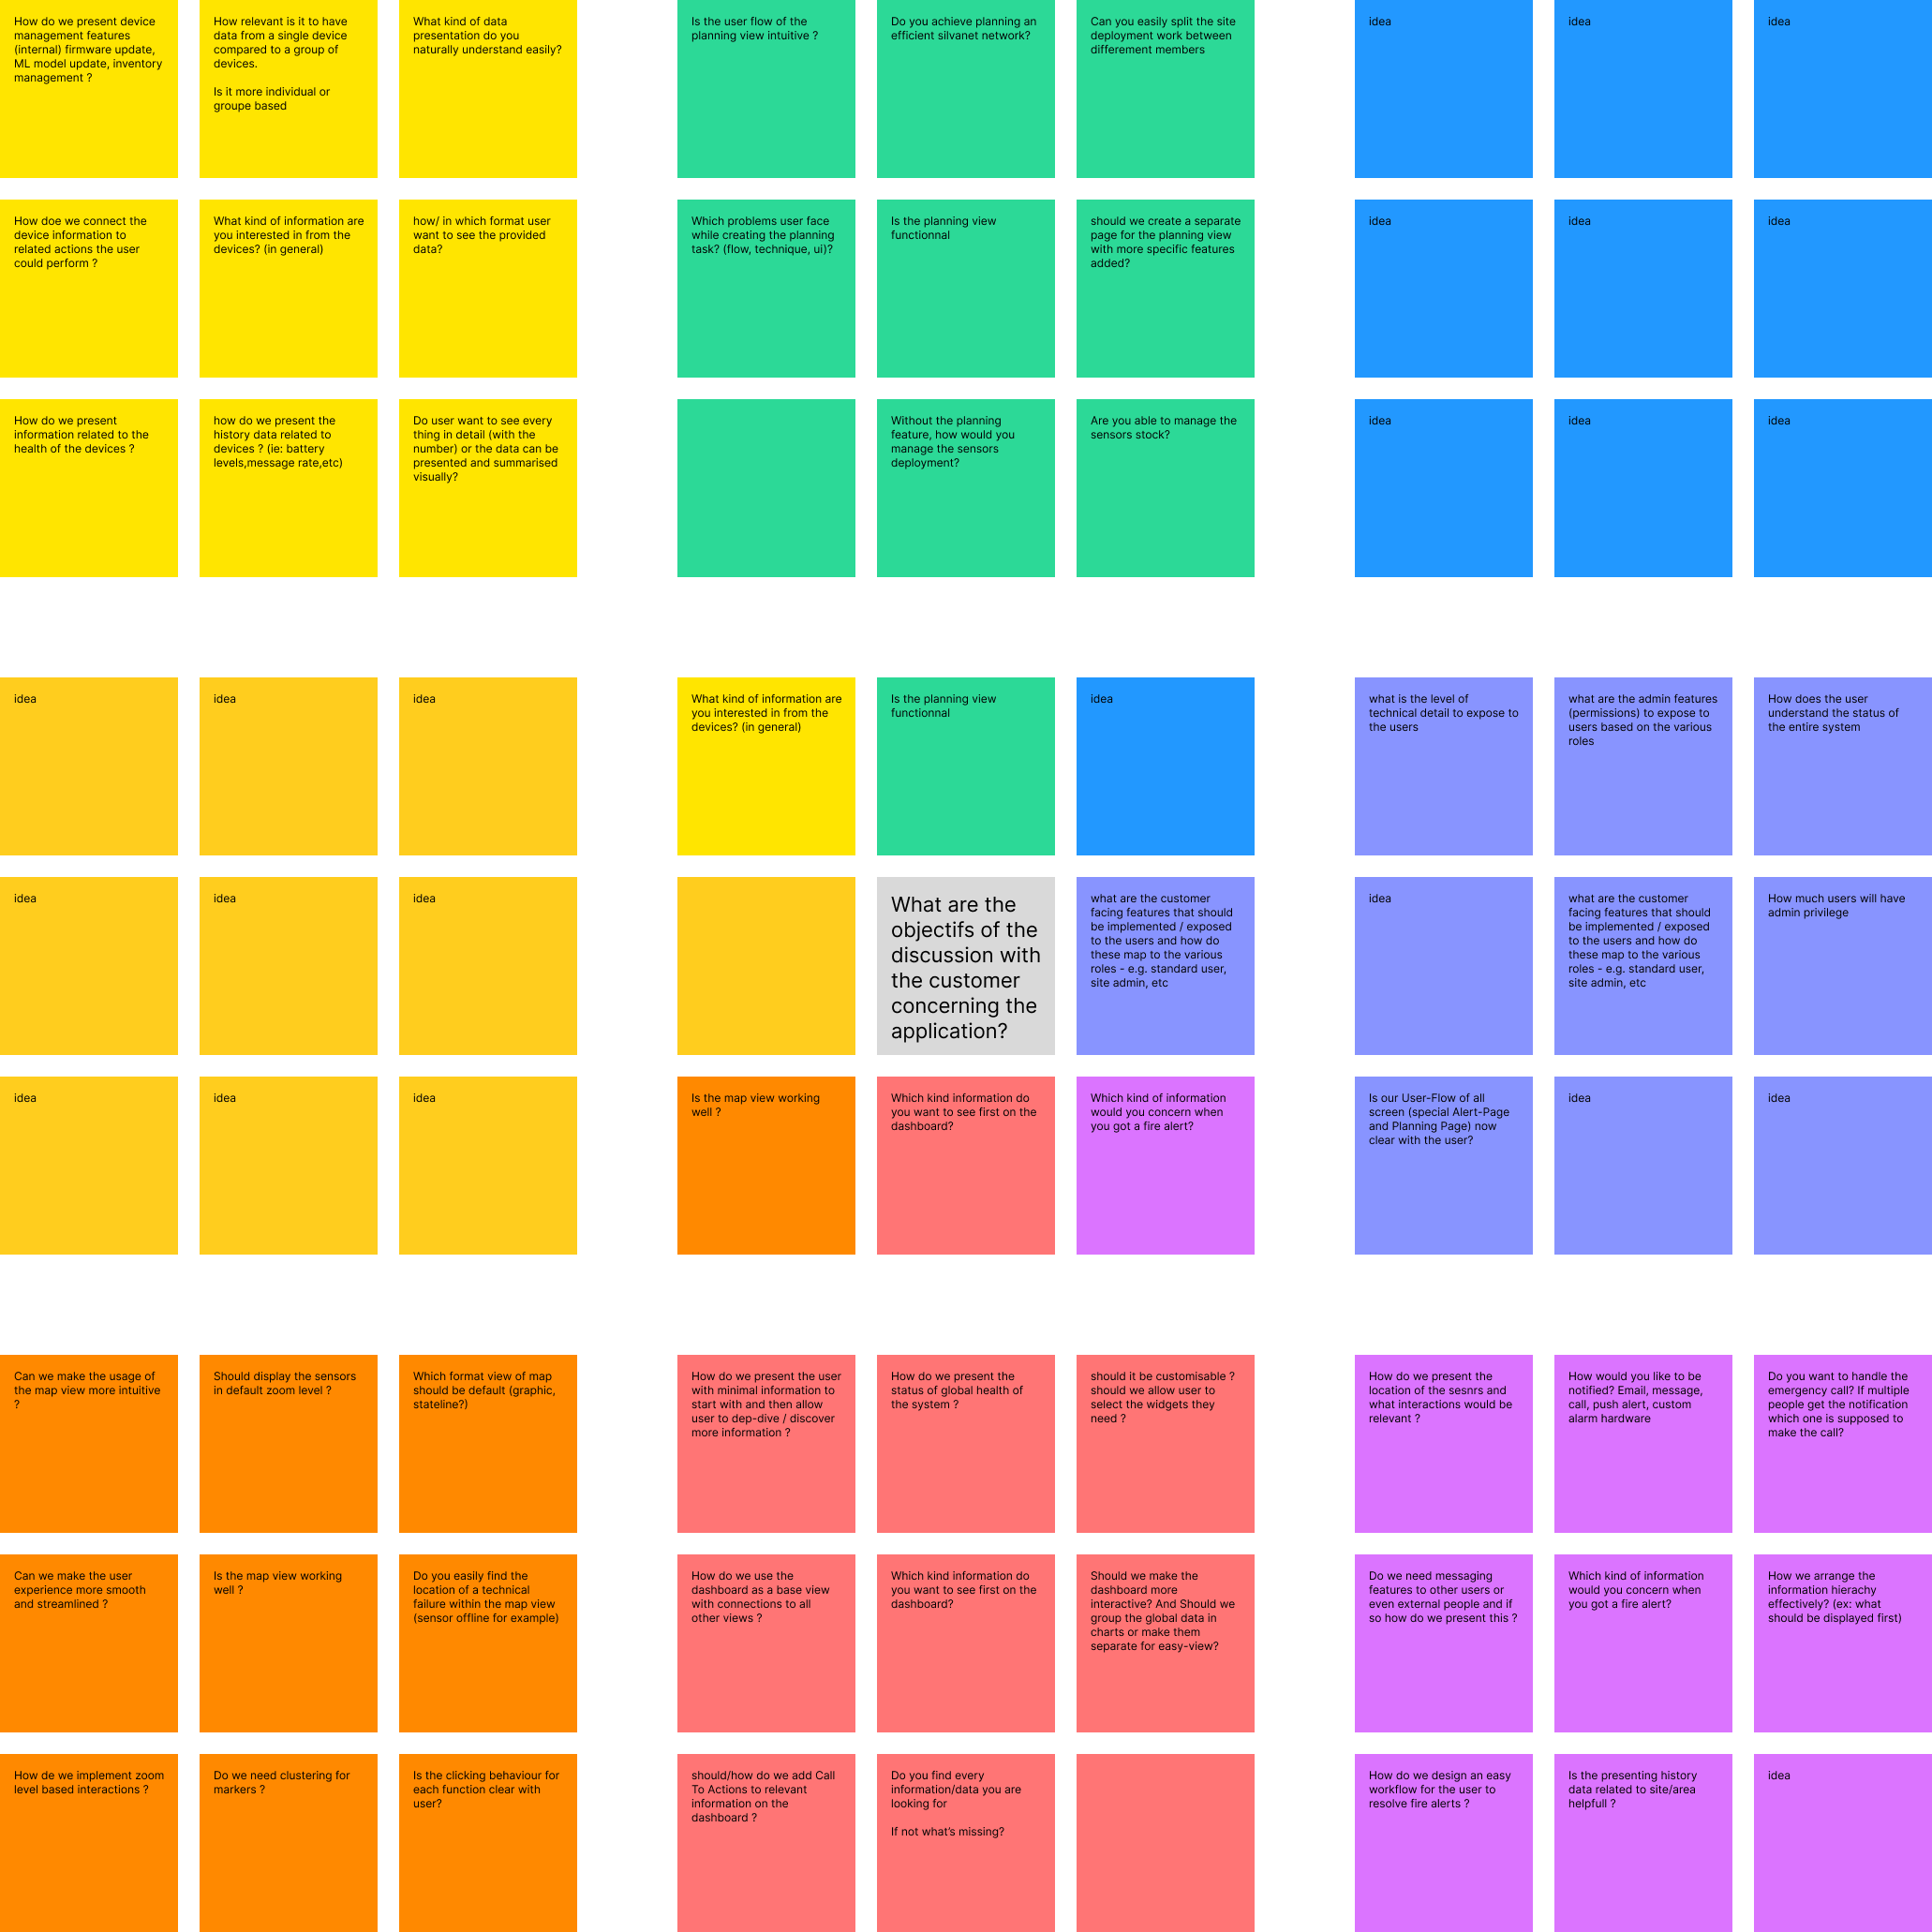
\includegraphics[width=\textwidth]{dryad_lotus_blossom_cycle_2}
  \caption{Durchführung des zweiten Ideationszyklus durch das Cloud-Team von Dryad mit der Lotus-Blossom-Methode}
  \label{fig:dryad_lotus_blossom_cycle_2}
\end{figure}

Die Einzelheiten zu den verschiedenen Blütenblättern der Lotus Blossom des zweiten Zyklus können im Anhang \ref{appendix:lotus_blossom} eingesehen werden.\\

Diese Aktivität ermöglichte es, die Usability-Tests schließlich auf die folgenden Features zu konzentrieren:

\begin{itemize}
  \item \textbf{Planung der Sensoren eines \textit{Site} \ac{UX}}: Die Anwendung bietet dem Nutzer eine Seite, auf der er auf einer interaktiven Karte die neuen Sensoren an einem \textit{Site} so positionieren kann, dass die Erfassungsabdeckung der Sensoren optimiert wird. Dies führt den Nutzer dann durch den Wald zu den Koordinaten, an denen er einen Sensor hoch oben an einem Baum befestigen muss.
  \item \textbf{Relevanz der Information in Alarmsituationen}: Wenn ein Feuer vom System erkannt wird, hat der Benutzer Zugang zu einer Alarmseite, die die Situation mithilfe von Daten und einer interaktiven Karte detailliert darstellt. Es sind auch schnelle Aktionen möglich, wie z.B. die Kontaktaufnahme mit den örtlichen Behörden. Dies betrifft auch Informationen, die per E-Mail an den Nutzer gesendet werden, um ihn über den Alarm zu benachrichtigen.
  \item \textbf{Usability der interaktiven Karte}: Die Anwendung bietet eine Seite, die nur aus einer interaktiven Karte besteht, auf der Sie die verschiedenen \textit{Sites} und Sensoren anhand ihrer geografischen Lage einsehen können.
  \item \textbf{Relevanz von Sensordaten}: In der Anwendung werden die Sensordaten auf unterschiedliche Weise dargestellt. Es wäre interessant, die Strategie zu definieren, die verwendet wird, um diese Daten für den Benutzer relevant zu präsentieren.
\end{itemize}

\subsection{Methoden für Usability-Tests}
